
\section{Testes}

Foram realizados diversos testes que estudam o impacto da variação do débito e do número de nós do sistema no tempo de
execução. Um conjunto de testes foi efetuado num modo que designamos por \textit{baseline}. 
Este consiste em eliminar toda a comunicação entre nós do sistema, visando analisar o \textit{overhead}
introduzido pela troca de mensagens (e consequentemente, da emulação da rede virtual). No entanto, a
actividade de geração e inserção de tuplos na base de dados é preservada, realizando-se um
número total equivalente de gerações e inserções de tuplos.


Em todos os testes foi fixado o fator de agregação ($AG = 100$), referido em \ref{benchs}, uma vez que se concluiu
que este parâmetro apenas é relevante para valores baixos (de 1 a 5).

Todos os testes foram executados em ambos os ambientes ({\conts} e VMs). Os parâmetros de teste são os seguintes:
\begin{itemize}

\item Variação de débito com 15 nós e todas as inserções locais (\textbf{teste 1}: {\conts}, $D$ variável, $N = 15$ e modo \textit{baseline})
\item Variação do número de nós com cada nó a gerar 5000 tuplos por minuto que insere $N$ vezes localmente (\textbf{teste 2}: {\conts}, $D$ = 5000, $N$ variável, e modo \textit{baseline})

\item Variação de débito (\textbf{teste 3}: {\conts}, $D$ variável, $N = 15$)
\item Variação do número (\textbf{teste 4}: {\conts}, $D$ = 5000, $N$ variável)

\end{itemize}

O comportamento esperado do sistema varia de acordo com o número de operações que este executa por unidade de tempo. Este número é,
no essencial, proporcional ao número de inserções na base de dados.
A equação que define o número total de inserções por unidade de tempo é a seguinte:

\begin{equation}
\label{eq:operacoes}
 I = N^2 * D
\end{equation}

% Sendo que N corresponde ao número de nós do \textit{benchmark} e D ao débito de geração de tuplos por nó.

\subsection{Resultados}

Nesta secção serão apresentados os resultados obtidos pelos testes apresentados acima. 
Cada gráfico relaciona o parâmetro que varia com o desvio (em percentagem) do tempo de execução esperado,
\ie o tempo definido pelo débito $D$ admitindo que as operações são realizadas sem atrasos.

	
\begin{figure}[h!]
	\centering
	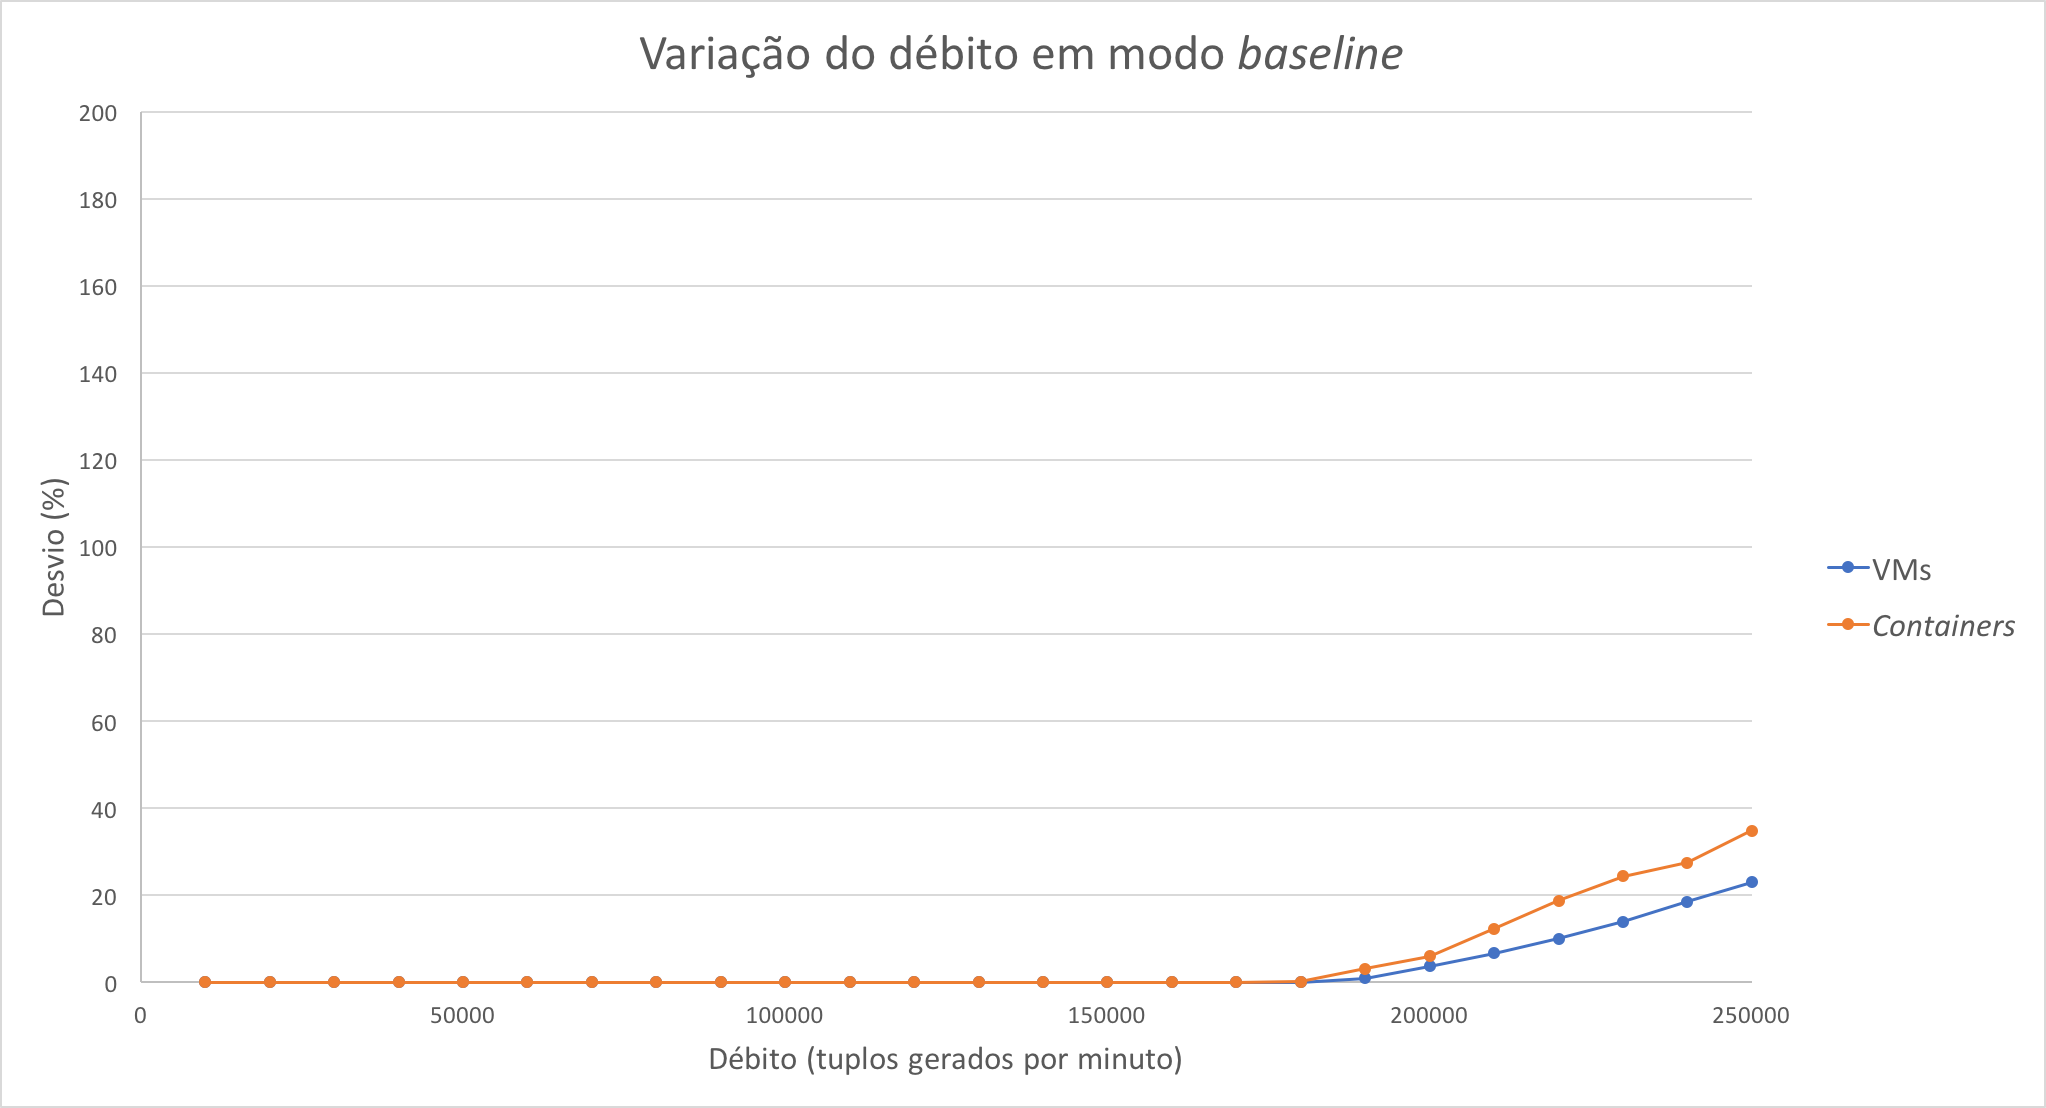
\includegraphics[width=0.9\linewidth]{figures/graphs/baseline_insertions}
	\caption{\textbf{Teste 1} ({\conts} e VMs, $D$ variável, $N = 15$ e modo \textit{baseline})}
	\label{fig:results-ins-baseline}
\end{figure}

\begin{figure}[h!]
	\centering
	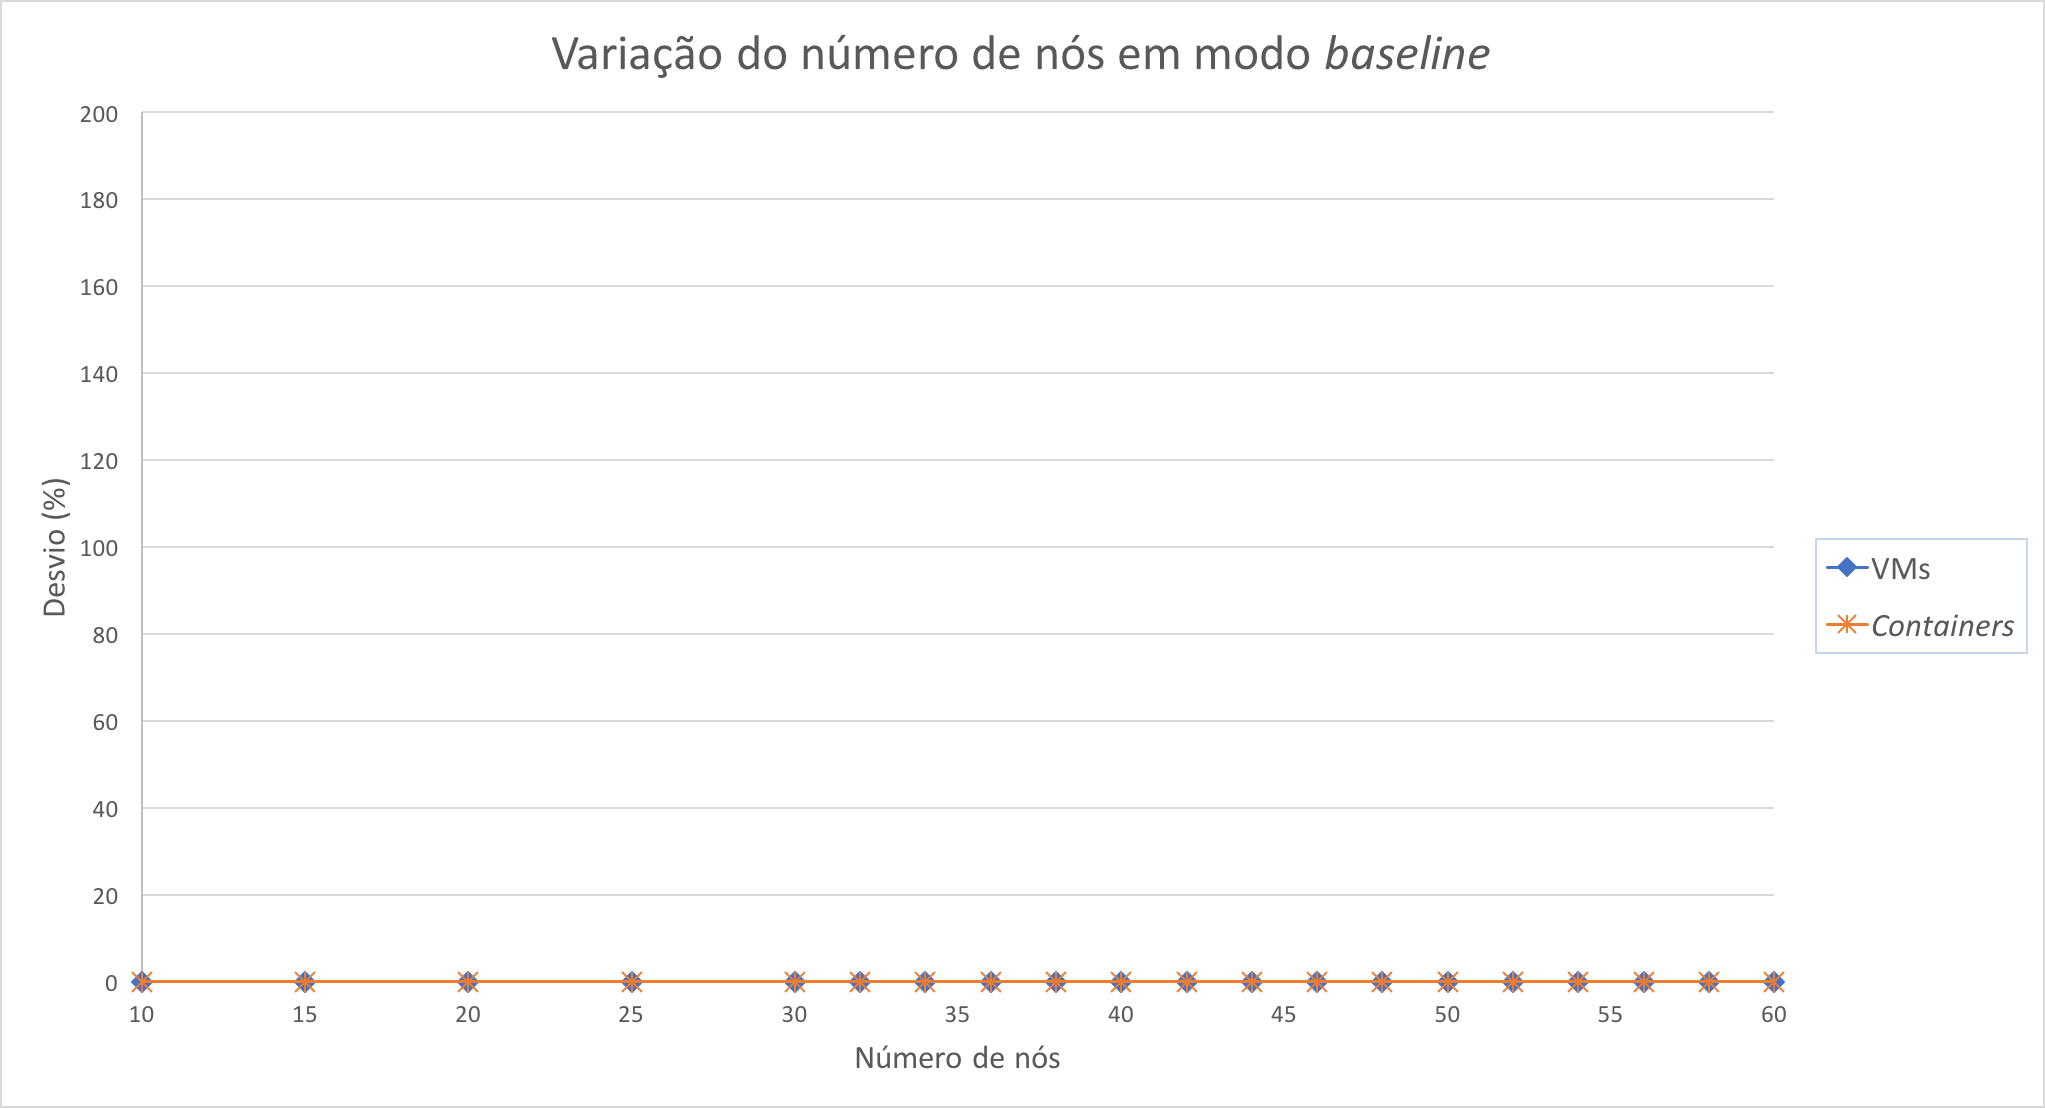
\includegraphics[width=0.9\linewidth]{figures/graphs/baseline_numNodes}
	\caption{\textbf{Teste 2} ({\conts} e VMs, $D = 5000$, $N$ variável, e modo \textit{baseline})}
	\label{fig:results-nos-baseline}
\end{figure}

\begin{figure}[h!]
	\centering
	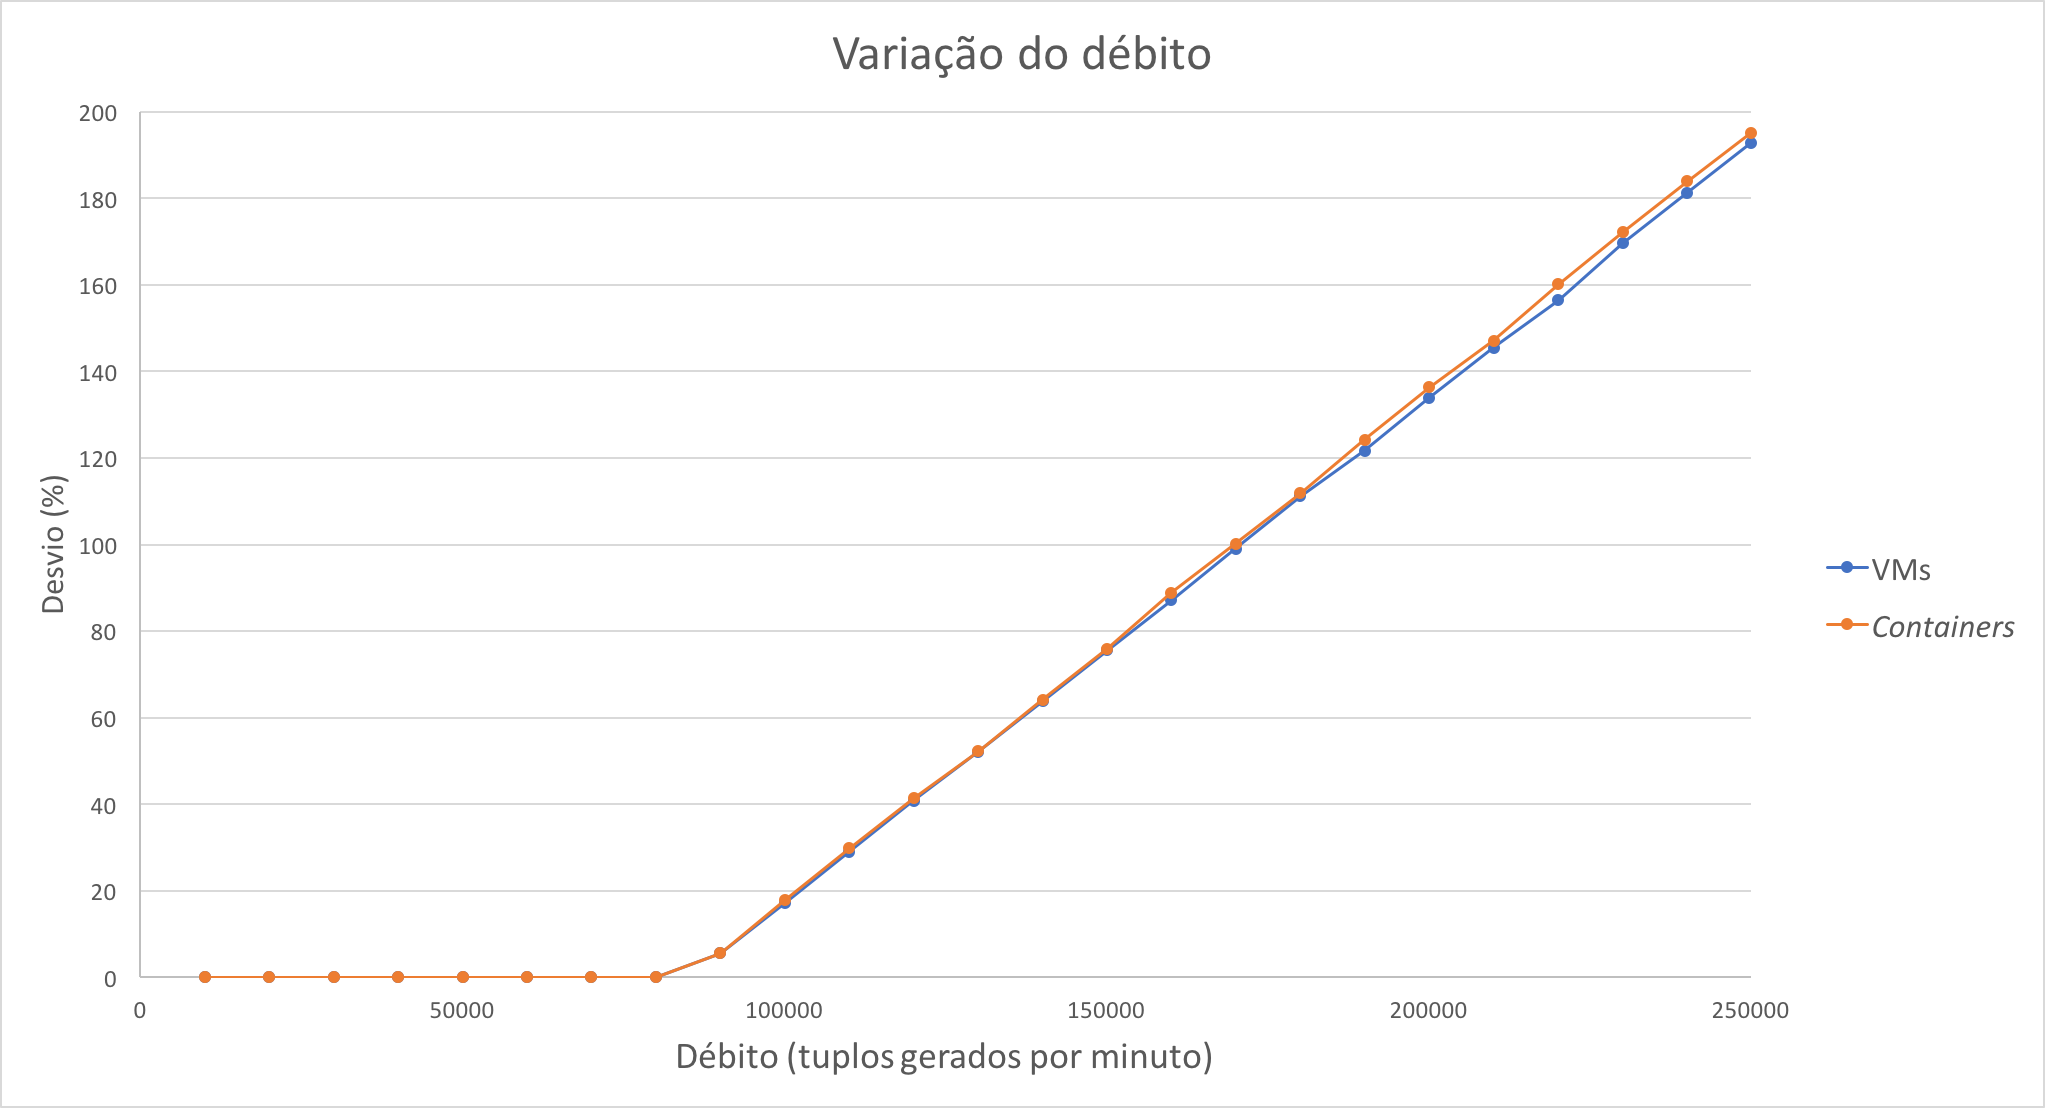
\includegraphics[width=0.9\linewidth]{figures/graphs/insertions}
	\caption{\textbf{Teste 3} ({\conts} e VMs, $D$ variável, $N = 15$)}
	\label{fig:results-insertions}
\end{figure}

\begin{figure}[h!]
	\centering
	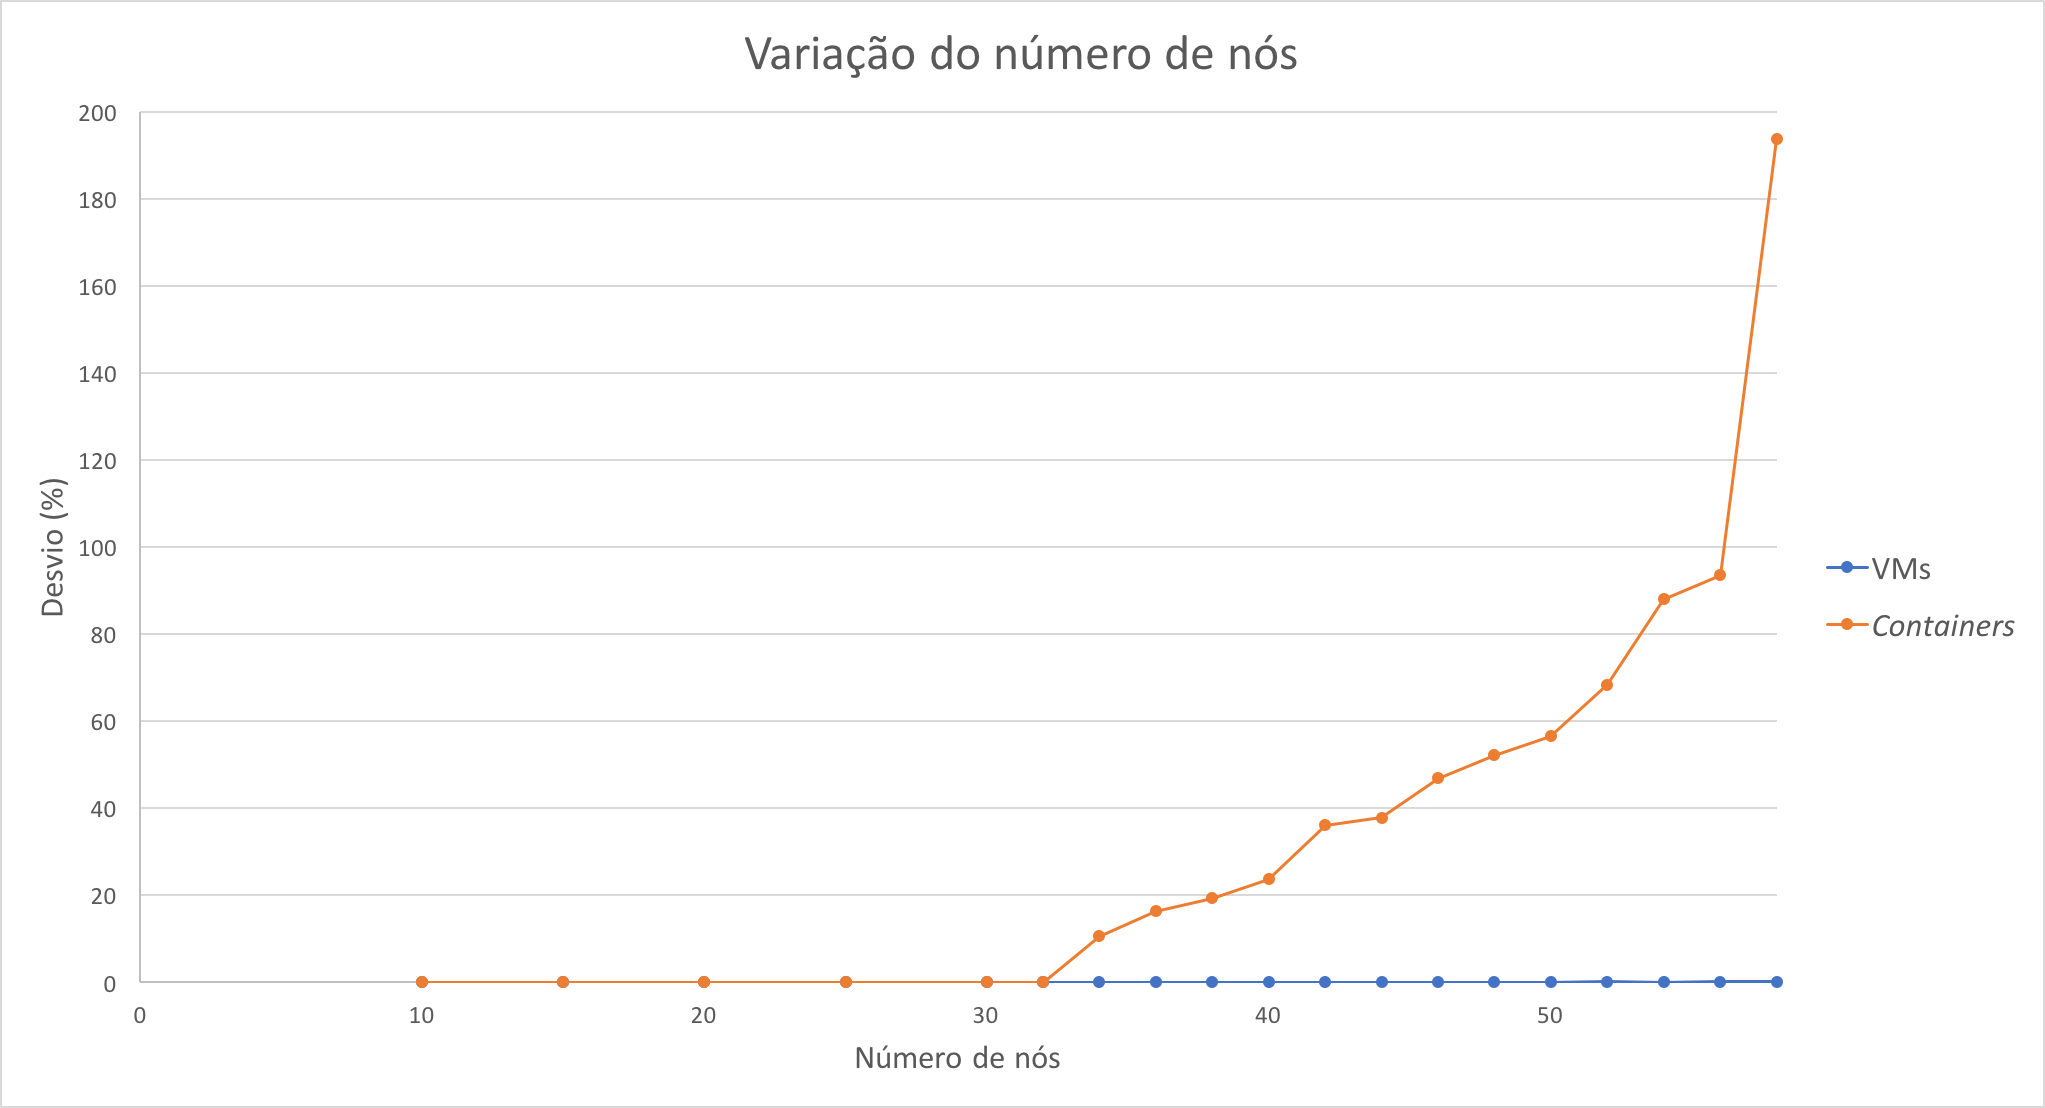
\includegraphics[width=0.9\linewidth]{figures/graphs/numNodes}
	\caption{\textbf{Teste 4} ({\conts} e VMs, $D = 5000$, $N$ variável)}
	\label{fig:results-nos}
\end{figure}

%Nas figuras \ref{fig:docker-ins} e \ref{fig:vms-ins} encontra-se representado o comportamento de ambos os ambientes de emulação fazendo variar as inserções por minuto. Pode-se então verificar que fixando o número de nós, os testes exibem um incremento linear, tal como esperado de acordo com a equação anteriormente apresentada. A diferença entre as duas soluções é insignificante.


%As figuras \ref{fig:docker-nos} e \ref{fig:vms-nos} apresentam os resultados dos testes em que se estuda o impacto da variação do número de instâncias. Verifica-se que no caso dos {\conts} o \textit{runtime} varia de acordo com o aumento de operações.

